\section*{Problem Statement} 
The objective of this problem is to solve the time-dependent Schrödinger equation numerically using the Gauss--Jordan elimination method. The wavefunction $\psi(t)$ evolves according to:
\[
i \hbar \frac{d\psi}{dt} = E \psi,
\]
where $E$ is the energy of the system. For a constant energy $E$, the analytical solution is an exponential function:
\[
\psi(t) = \psi(0) \, e^{-iEt/\hbar}.
\]
The aim is to discretize this equation, solve the resulting linear system using Gauss--Jordan elimination, and study both the magnitude and phase of $\psi(t)$ over time.

\section*{Methodology} 
The differential equation is discretized using finite differences. With time step $\Delta t$, the recursion can be expressed as:
\[
\psi_k - \delta \, \psi_{k-1} = R_k, \quad k=2,3,\dots,N,
\]
where
\[
\delta = \frac{iE\Delta t}{\hbar} - 1.
\]

This leads to a system of linear equations $M \cdot \vec{\psi} = \vec{R}$, where:
\begin{itemize}
  \item $M$ is a bidiagonal matrix with $M(k,k)=1$ and $M(k,k-1)=\delta$ for $k \geq 2$,
  \item $\vec{R}$ is the right-hand side vector incorporating the initial condition $\psi(0) = \psi_0$.
\end{itemize}

\subsection*{Algorithm}
\begin{enumerate}
  \item Define parameters: $\Delta t$, $t_{\max}$, $\hbar$, $E$, and $\psi_0$.
  \item Construct coefficient matrix $M$ and vector $\vec{R}$.
  \item Form augmented matrix $A = [M|\vec{R}]$.
  \item Apply Gauss--Jordan elimination to reduce $A$ to diagonal form:
  \[
  A(r,:) = A(r,:) - \frac{A(r,p)}{A(p,p)} \cdot A(p,:), \quad r \neq p.
  \]
  \item Extract solution $\psi_k = A(k,end)/A(k,k)$ for all $k$.
  \item Plot $|\psi(t)|$ (magnitude) and $\arg(\psi(t))$ (phase) versus time.
\end{enumerate}

\section*{Results} 
The chosen parameters are:
\[
\Delta t = 0.01, \quad t_{\max} = 5.0, \quad \hbar = 6.626 \times 10^{-34}, \quad E = -10\hbar, \quad \psi_0 = 0.5 + 0.5i.
\]

The numerical solution $\psi(t)$ was computed at discrete time steps. Figure~\ref{fig:schrodinger} shows the evolution of the wavefunction.

\begin{figure}[h!]
  \centering
  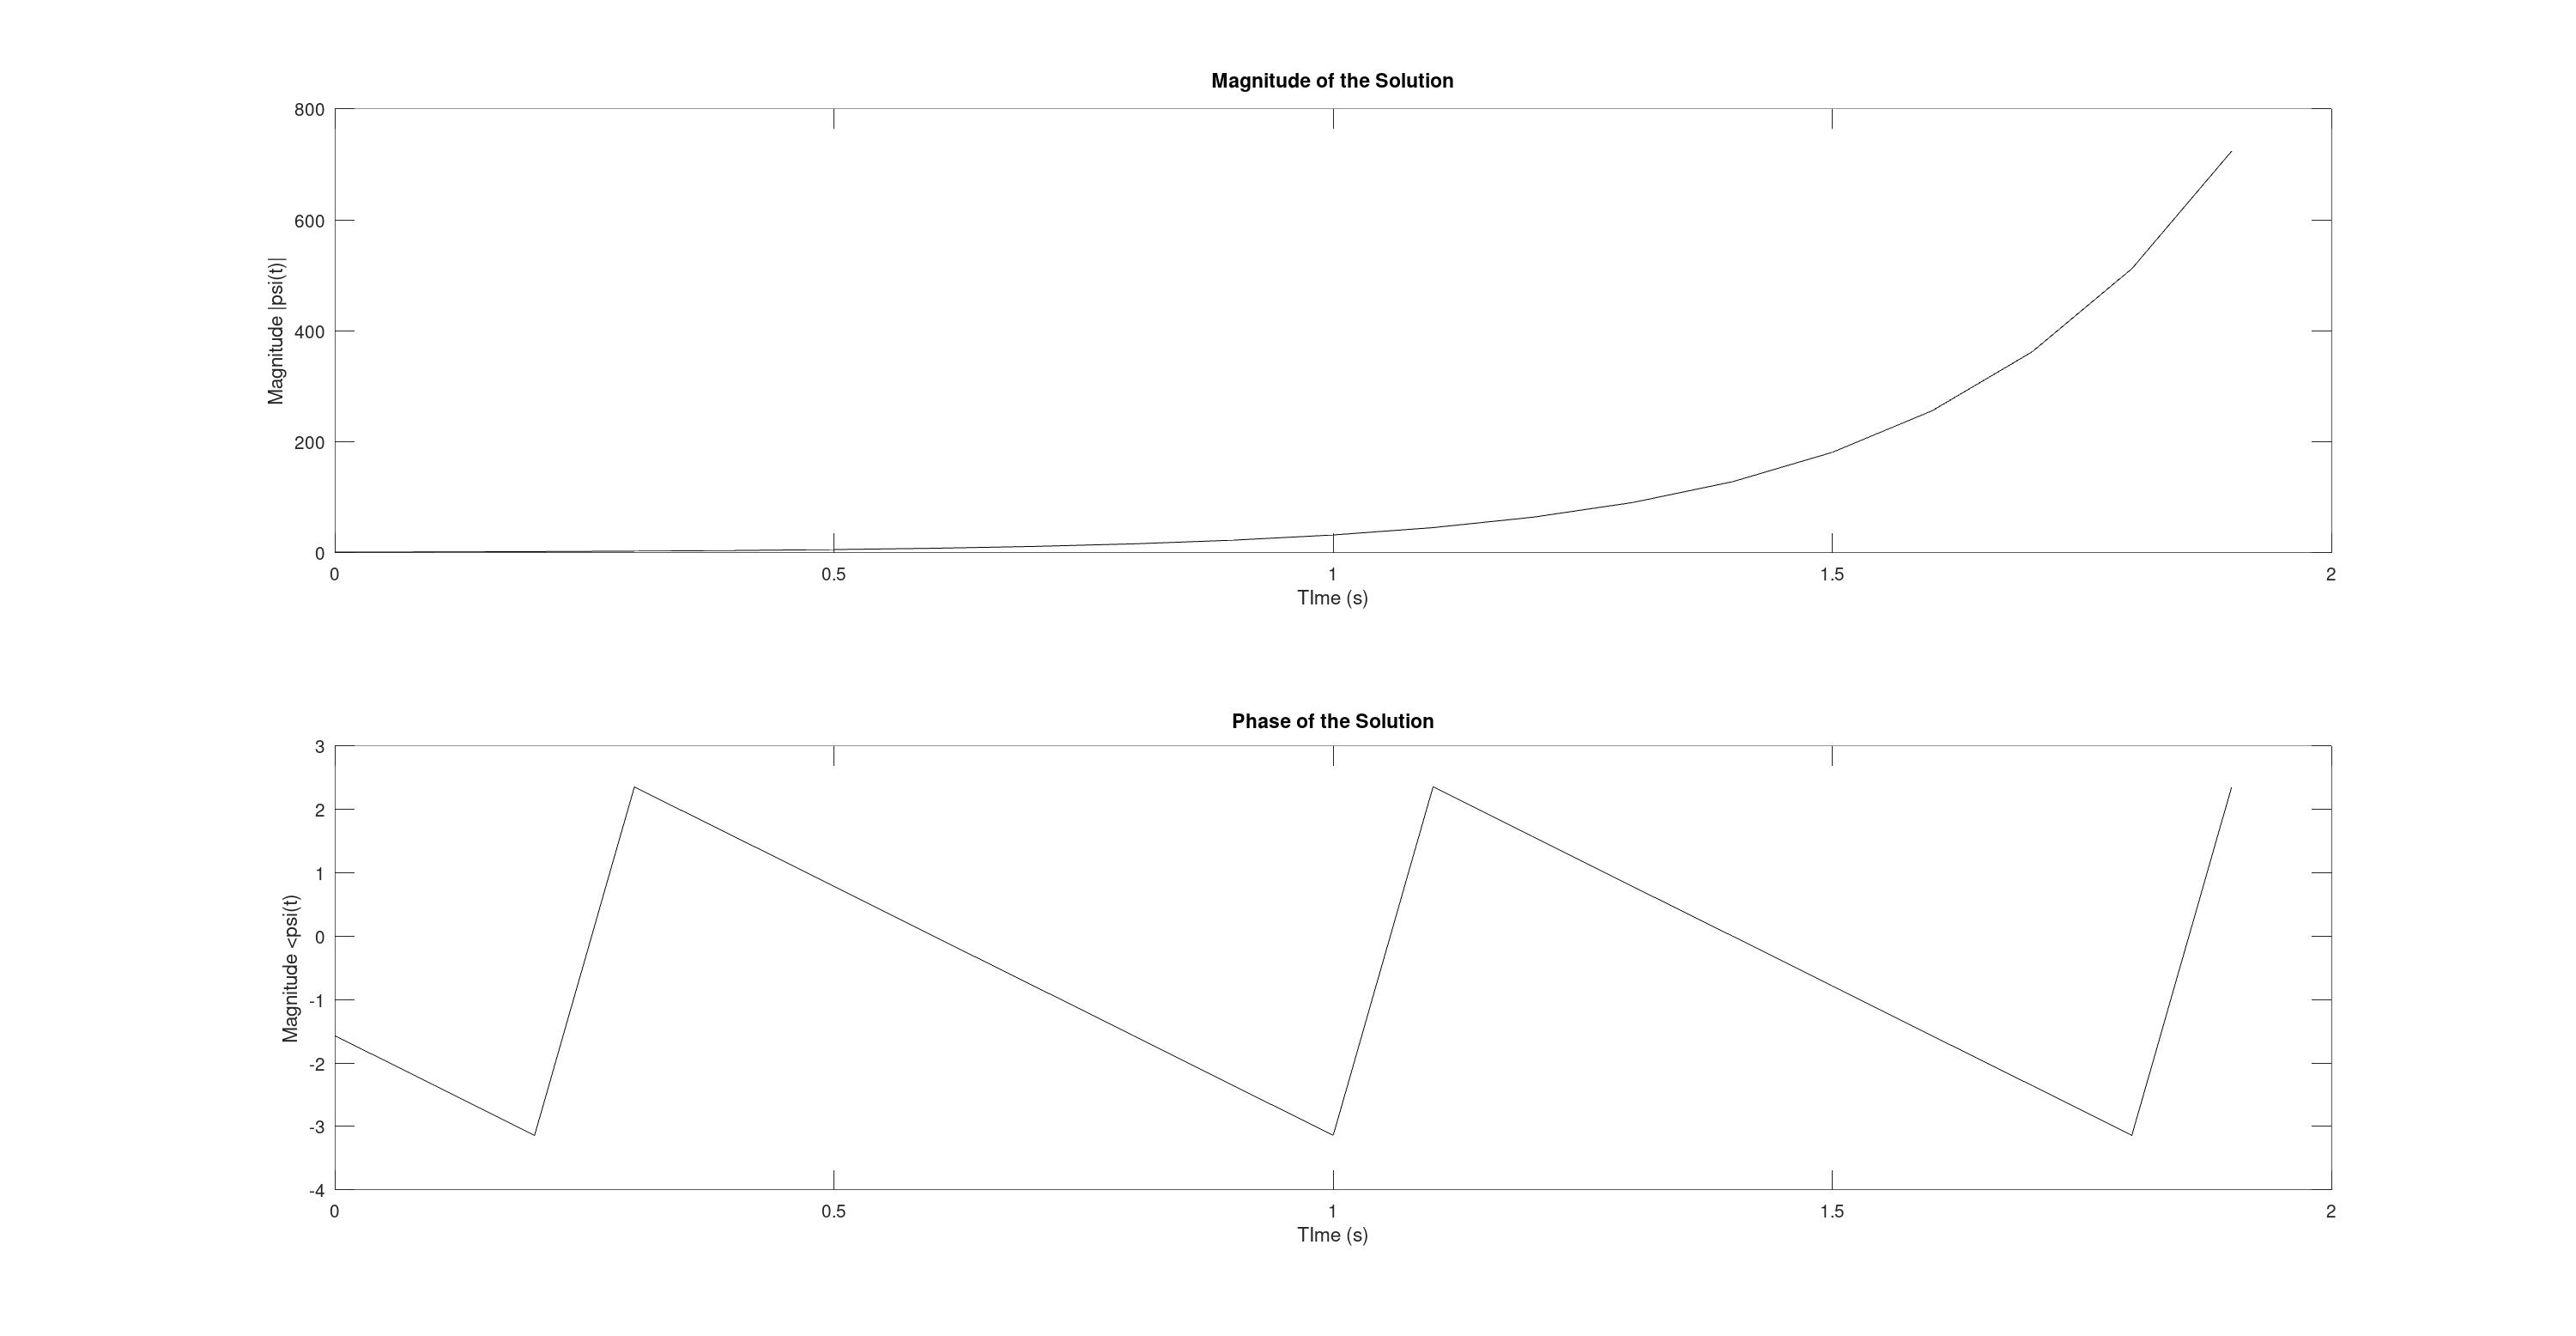
\includegraphics[width=0.8\textwidth]{a5.jpg}
  \caption{Time evolution of the wavefunction $\psi(t)$: (top) magnitude $|\psi(t)|$, (bottom) phase $\arg(\psi(t))$.}
  \label{fig:schrodinger}
\end{figure}

The observed behavior is:
\begin{itemize}
  \item The magnitude $|\psi(t)|$ does not remain perfectly constant, but instead drifts over time.
  \item The phase $\arg(\psi(t))$ roughly follows a linear increase, though small deviations accumulate.
\end{itemize}

These deviations are not physical but arise from \textbf{numerical round-off errors} introduced by the Gauss--Jordan elimination method and the discretization scheme. Since the matrix system is ill-conditioned, the method does not preserve the unitarity of Schrodinger evolution.

\section*{Conclusion} 
The Gauss--Jordan elimination method was applied to the time-dependent Schrödinger equation for a constant-energy system. While the analytical solution predicts constant magnitude and a linearly increasing phase, the numerical results show noticeable deviations.  

This discrepancy highlights a limitation of the chosen numerical scheme: round-off errors accumulate, and the method does not enforce unitarity. Therefore, although Gauss--Jordan elimination demonstrates how linear algebra techniques can be applied.
